\documentclass[a4paper, 12pt]{report}
\usepackage{cmap}
\usepackage[T2A]{fontenc}
\usepackage[utf8]{inputenc}
\usepackage[english,russian]{babel}
\usepackage{listings}
\usepackage{amsmath}
\usepackage{float}
\usepackage{csquotes}
\usepackage{graphicx}
\graphicspath{ {./images/} }
\usepackage{xcolor}
\definecolor{buzzlightyear}{HTML}{8757A5}
\definecolor{grass}{HTML}{738D06}
\definecolor{literal}{HTML}{F18A2B}
\definecolor{commentcolor}{HTML}{8E908B}

\lstdefinestyle{habrstyle}{
	backgroundcolor=\color{white},
	commentstyle=\color{commentcolor},
	keywordstyle=\bfseries\color{buzzlightyear},
	numberstyle=\tiny\color{commentcolor},
	stringstyle=\color{grass},
	basicstyle=\ttfamily\footnotesize,
	breakatwhitespace=false,         
    	breaklines=true,                 
   	captionpos=b,                    
    	keepspaces=true,                 
    	numbers=left,                    
    	numbersep=7pt,                  
    	showspaces=false,                
    	showstringspaces=false,
   	showtabs=false,                  
    	tabsize=4
}

\lstset{style=habrstyle}

\author{3530901/80201, Шелаев Н. Р.}
\title{Лабораторная работа № 1. Звуки и сигналы.}
\date{\today}

\begin{document}
	\maketitle
	\tableofcontents
	\listoffigures
	\lstlistoflistings

	\chapter{Периодические сигналы}
	Строим периодические сигналы.
	\begin{lstlisting}[language=Python,caption=Построение сигнала \texttt{Cos} и  \texttt{Sin} и их суммы]
		from thinkdsp import CosSignal, SinSignal
		cos_sig = CosSignal(freq=440, amp=1.0, offset=0)
		sin_sig = SinSignal(freq=880, amp=0.5, offset=0)
		mix = sin_sig + cos_sig
	\end{lstlisting}
	\begin{figure}[H]
		\centering
		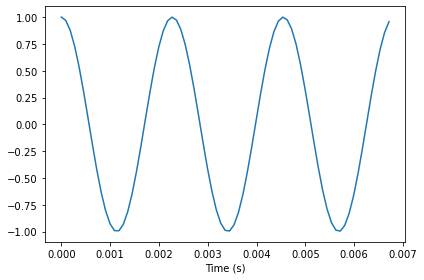
\includegraphics[width=0.75\textwidth]{cos.png}
		\caption{Косинусоида}
		\label{fig:cos}
	\end{figure}
	\begin{figure}[H]
		\centering
		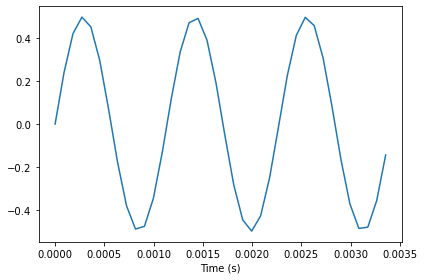
\includegraphics[width=0.75\textwidth]{sin.png}
		\caption{Синусоида}
		\label{fig:sin}
	\end{figure}
	\begin{figure}[H]
		\centering
		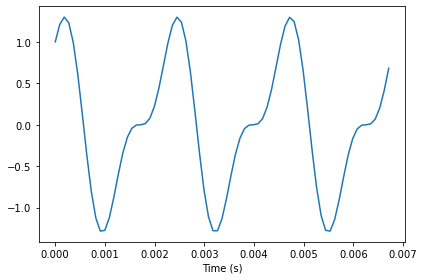
\includegraphics[width=0.75\textwidth]{mix.png}
		\caption{Сумма двух сигналов}
		\label{fig:mix}
	\end{figure}
	
	\chapter{Получение звука}
	Знакомимся с некоторыми функциями предоставленного нам класса  \texttt{wave} для получения сигналов и их первичной обработки.
	\begin{lstlisting}[language=Python,caption=Получение сигнала]
		wave = mix.make_wave(duration = 0.5, start = 0, framerate = 11025)
		period = mix.period
		segment = wave.segment(start=0, duration=period * 3)
		segment.plot()
		wave.normalize()
		wave.apodize()
		wave.plot()
	\end{lstlisting}
	Результаты для суммы \texttt{Cos} и  \texttt{Sin}:
	\begin{figure}[H]
		\centering
		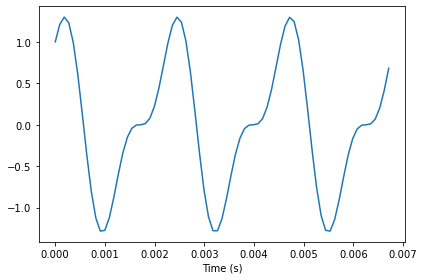
\includegraphics[width=0.75\textwidth]{segment_mix.png}
		\caption{Небольшой сегмент сигнала (3 периода)}
		\label{fig:segment_mix}
	\end{figure}
	\begin{figure}[H]
		\centering
		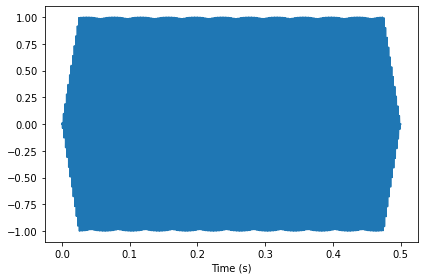
\includegraphics[width=0.75\textwidth]{wave_mix.png}
		\caption{Нормализованный сигнал}
		\label{fig:wave_mix}
	\end{figure}
	Также мы можем сигнал из WAV файлов.
	\begin{lstlisting}[language=Python,caption=Получение сигнала]
		from thinkdsp import read_wave
		wave = read_wave('92002__jcveliz__violin-origional.wav')	
		wave.make_audio()
		segment = wave.segment(start = 1.2, duration = 0.6)
		segment.plot()
	\end{lstlisting}
	\begin{figure}[H]
		\centering
		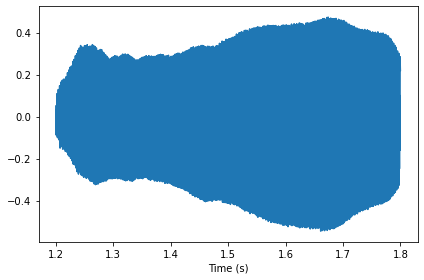
\includegraphics[width=0.75\textwidth]{segment_file.png}
		\caption{Сегмент сигнала из  WAV файла}
		\label{fig:segment_file}
	\end{figure}

	\chapter{Спектр сигнала}
	Строим спектр сигнал.
	\begin{lstlisting}[language=Python,caption=Спектр сигнала]
		spectrum = segment.make_spectrum()
		spectrum.plot()
	\end{lstlisting}
	\begin{figure}[H]
		\centering
		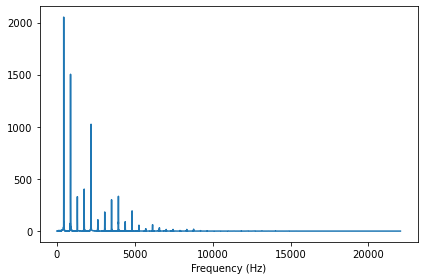
\includegraphics[width=0.75\textwidth]{spectrum1.png}
		\caption{Полученный спектр сигнала}
		\label{fig:spectrum1}
	\end{figure}
	Частотные составляющие выше 10 кГц достаточно малы, поэтому мы можем лучше рассмотреть нижние частоты.
	\begin{lstlisting}[language=Python,caption=Улучшаем масштаб]
		spectrum.plot(high = 10000)
	\end{lstlisting}
	\begin{figure}[H]
		\centering
		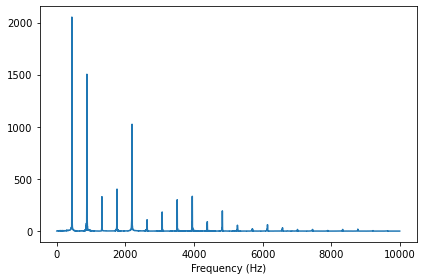
\includegraphics[width=0.75\textwidth]{spectrum2.png}
		\caption{Так уже лучше}
		\label{fig:spectrum2}
	\end{figure}

	\chapter{Фильтрация}
	Исследуем работу различных фильтров.
	\begin{lstlisting}[language=Python,caption=Функция для фильтра нижних частот]
		spectrum.low_pass(3000)
		spectrum.plot(high = 10000)
		filtered = spectrum.make_wave()
		filtered.normalize()
		filtered.apodize()
		filtered.plot()
		segment.normalize()
		segment.apodize()
		segment.plot()
	\end{lstlisting}
	\begin{figure}[H]
		\centering
		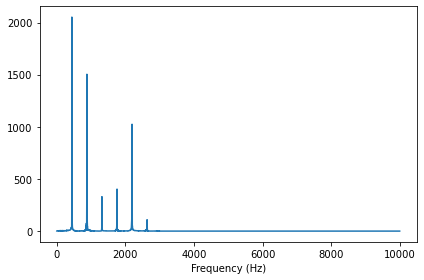
\includegraphics[width=0.75\textwidth]{spectrum3.png}
		\caption{Спектр сигнала с применением фильтра нижних частот}
		\label{fig:spectrum3}
	\end{figure}
	\begin{figure}[H]
		\centering
		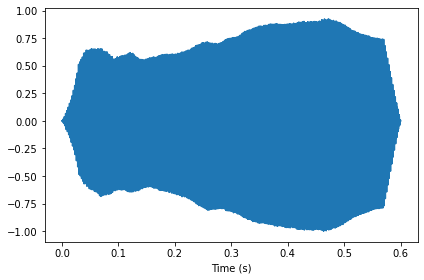
\includegraphics[width=0.75\textwidth]{wave_filter.png}
		\caption{Отфильтрованный сигнал}
		\label{fig:wave_filter}
	\end{figure}
	\begin{figure}[H]
		\centering
		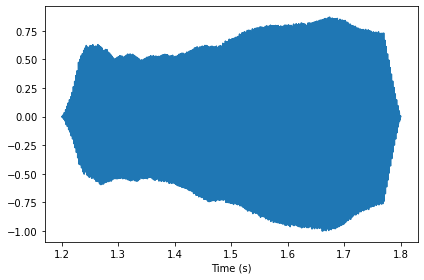
\includegraphics[width=0.75\textwidth]{segment_filter.png}
		\caption{Оригинальный сигнал}
		\label{fig:segment_filter}
	\end{figure}
	При их прослушивании отфильтрованная версия сигнала звучит более однотонно и с приглушенным качеством. Этот сигнал слышится как оригинальный, как если бы его воспроизводили по телефону или через стену.

	\chapter{Упражнения}
	\section{Задание 2}
	Применяем различные фильтры для сложного сигнала.
	\begin{lstlisting}[language=Python,caption=Получение сложного сигнала]
		wave = read_wave('170255__dublie__trumpet.wav')
		wave.normalize()
		wave.plot()
	\end{lstlisting}
	\begin{figure}[H]
		\centering
		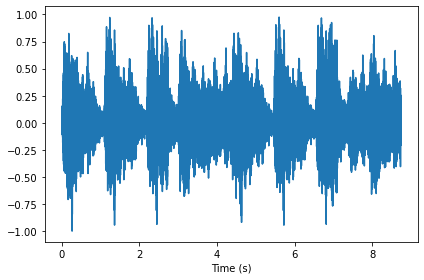
\includegraphics[width=0.75\textwidth]{wave1.png}
		\caption{Сложный сигнал}
		\label{fig:wave1}
	\end{figure}
	\begin{lstlisting}[language=Python,caption=Сегмент сигнала]
		segment = wave.segment(start = 2.2, duration = 0.4)
		segment.plot()
	\end{lstlisting}
	\begin{figure}[H]
		\centering
		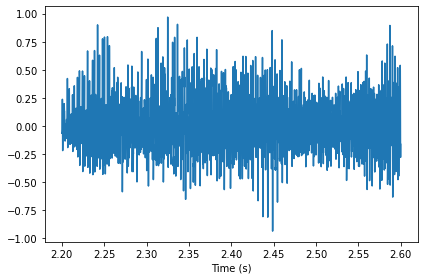
\includegraphics[width=0.75\textwidth]{wave2.png}
		\caption{Взяли небольшой сегмент сигнала}
		\label{fig:wave2}
	\end{figure}
	\begin{lstlisting}[language=Python,caption=Получение спектра сигнала]
		segment = wave.segment(start = 2.2, duration = 0.4)
		segment.plot()
	\end{lstlisting}
	\begin{figure}[H]
		\centering
		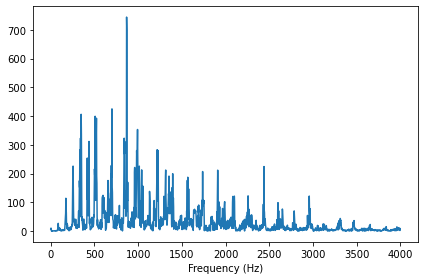
\includegraphics[width=0.75\textwidth]{spectrum4.png}
		\caption{Спектр сигнала}
		\label{fig:spectrum4}
	\end{figure}
	\begin{lstlisting}[language=Python,caption=Улучшаем масштаб спектра]
		spectrum = segment.make_spectrum()
		spectrum.plot(high = 1000)
	\end{lstlisting}
	\begin{figure}[H]
		\centering
		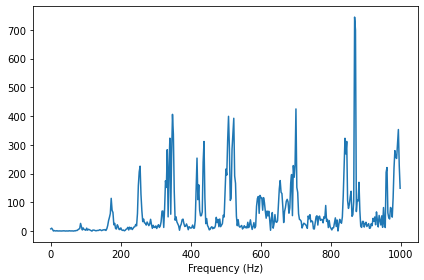
\includegraphics[width=0.75\textwidth]{spectrum5.png}
		\caption{Так лучше видны пики спектра}
		\label{fig:spectrum5}
	\end{figure}
	\begin{lstlisting}[language=Python,caption=Находим основную частоту сигнала (основной пик спектра)]
		spectrum = segment.make_spectrum()
		spectrum.plot(high = 100)
	\end{lstlisting}
	\begin{figure}[H]
		\centering
		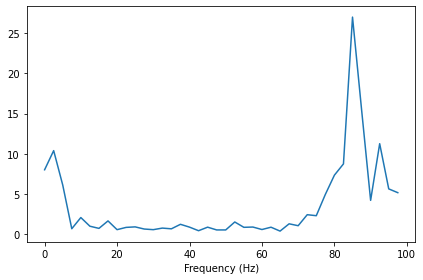
\includegraphics[width=0.75\textwidth]{spectrum6.png}
		\caption{Основная частота сигнала}
		\label{fig:spectrum6}
	\end{figure}
	Доминирующий пик находится на частоте 867,5 Гц. Основной пик составляет примерно 85,0 Гц с гармониками 170, 255, 340, 425, 510, ... Гц.  Высота тона сигнала, которую мы воспринимаем, обычно является фундаментальной, даже если она не является доминантной.
	\begin{lstlisting}[language=Python,caption=Функция фильтра НЧ]
		from ipywidgets import interact, fixed

		def filter_wave_low(wave, low, factor):
    			segment = wave.segment(2.2, 0.4)
   			spectrum = segment.make_spectrum()
    			spectrum.plot(high = 2500, color = '0.7')
    			spectrum.low_pass(low, factor)
    			spectrum.plot(high = 2500, color = '#045a8d')
    			decorate(xlabel = 'Frequency (Hz)')
    			audio = spectrum.make_wave().make_audio()
    			display(audio)

		interact(filter_wave_low, wave = fixed(wave), low = (0, 2500, 250), factor = (0, 1, 0.05));   
	\end{lstlisting}
	\begin{figure}[H]
		\centering
		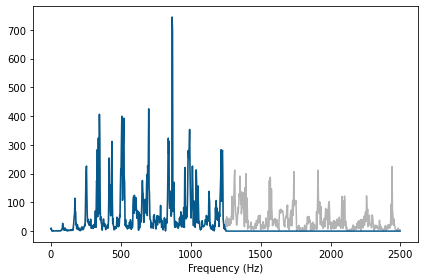
\includegraphics[width=0.75\textwidth]{filter1.png}
		\caption{Применение фильтра НЧ}
		\label{fig:filter1}
	\end{figure}
	Функции для фильтра верхних частот (ФВЧ) и полосо-заграждающего фильтра (ФПЗ) очень похожи на функцию для ФНЧ и поэтому здесь не приводятся.
	\begin{figure}[H]
		\centering
		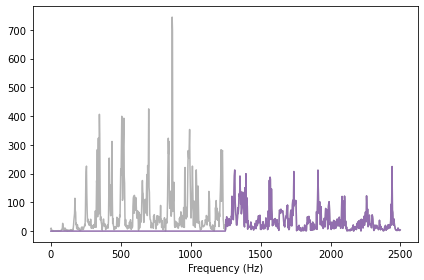
\includegraphics[width=0.75\textwidth]{filter2.png}
		\caption{Применение ФВЧ}
		\label{fig:filter2}
	\end{figure}
	\begin{figure}[H]
		\centering
		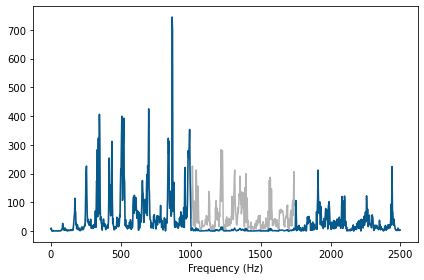
\includegraphics[width=0.75\textwidth]{filter3.png}
		\caption{Применение ФПЗ}
		\label{fig:filter3}
	\end{figure}

	\section{Задание 3}
	Создаём сложный сигнал и исследуем его.
	\begin{lstlisting}[language=Python,caption=Получение сложного сигнала через сумму других сигналов]
		import math
		signal = (SinSignal(freq = 600, amp = 0.4, offset = math.pi / 2) + CosSignal(freq = 200, amp = 0.6, offset = math.pi / 3) + SinSignal(freq = 800, amp = 0.8, offset = math.pi / 4) + CosSignal(freq = 400, amp = 1.0, offset = math.pi / 5))
		signal.plot()
	\end{lstlisting}
	\begin{figure}[H]
		\centering
		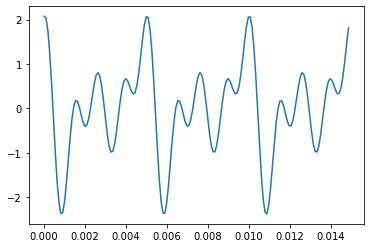
\includegraphics[width=0.75\textwidth]{sum.png}
		\caption{Полученный сложный сигнал}
		\label{fig:sum}
	\end{figure}
	\begin{lstlisting}[language=Python,caption=Спектр этого сигнала]
		wave = signal.make_wave(duration = 2.5)
		wave.apodize()
		spectrum = wave.make_spectrum()
		spectrum.plot(high = 1000)
	\end{lstlisting}
	\begin{figure}[H]
		\centering
		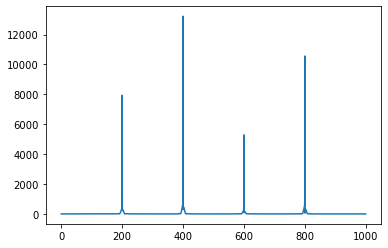
\includegraphics[width=0.75\textwidth]{spectrum7.png}
		\caption{Спектр сигнала с кратной частотой}
		\label{fig:spectrum7}
	\end{figure}
	Здесь использовались сигналы с частотой, кратной основным (что видно на спектре). Теперь добавим частотные компоненты, не кратные основным.
	 \begin{lstlisting}[language=Python,caption=Добавление некратной частоты]
		signal += SinSignal(freq = 500, amp = 0.7)
		wave = signal.make_wave(duration = 2.5)
		wave.apodize()
		spectrum = wave.make_spectrum()
		spectrum.plot(high = 1000)
	\end{lstlisting}
	\begin{figure}[H]
		\centering
		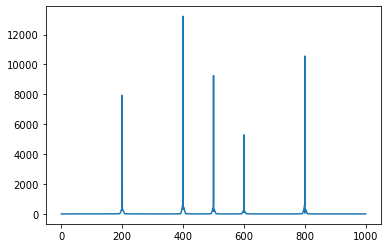
\includegraphics[width=0.75\textwidth]{spectrum8.png}
		\caption{Спектр с некратной частотой}
		\label{fig:spectrum8}
	\end{figure}
	Звук исходного сигнала изменился.
	
	\section{Задание 4}
	Функция \texttt{scretch} для ускорения и замедления сигнала.
	 \begin{lstlisting}[language=Python,caption=Функция для ускорения / замедления сигнала]
		wave = read_wave('170255__dublie__trumpet.wav')
		wave.normalize()

		def stretch(wave, speed_factor):
   			wave.ts /= speed_factor
   			wave.framerate *= speed_factor

		stretch(wave, 2)
		wave.plot()
	\end{lstlisting}
	\begin{figure}[H]
		\centering
		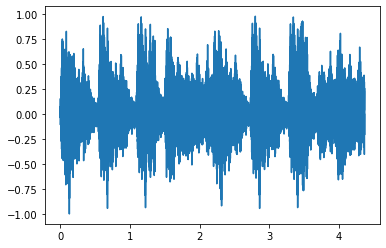
\includegraphics[width=0.75\textwidth]{result.png}
		\caption{Ускорение сигнала в 2 раза}
		\label{fig:result}
	\end{figure}

	\chapter{Вывод}
	В данной работе мы познакомились с функциями для первичной обработки сигналов. Построили сложный сигнал с некратной частотой и нашли его спектр. Также провели исследование действия различных фильтров на сигнал.
\end{document}